\documentclass[12pt]{article}
\usepackage{graphicx}
\usepackage{amsfonts}
\usepackage{amsmath}
\usepackage{amssymb}
\usepackage{enumitem}
\usepackage{xcolor}

\usepackage[a4paper, margin=1in]{geometry}

\setlength{\headheight}{15pt}
\usepackage{fancyhdr}
\pagestyle{fancy}
\fancyhf{}
\fancyhead[L]{CPSC/EENG 420 - Lab Report 2}
\fancyhead[R]{Bryan SebaRaj  \thepage}

\linespread{1.3} 

\title{Lab 2: Pipelined PARCv2 Processor}
\author{Bryan SebaRaj \\[0.5em] Professor Abhishek Bhattacharjee \\[0.5em] EENG 420 - Computer Architecture}
\date{February 21, 2025}

\begin{document}

\maketitle

% Abstract: introductory paragraph summarizing the lab
% • Design: describe your implementation, justifications for design decisions (if any), deviations from the
% prescribed datapath, discussion of any extensions
% • Testing Methodology: describe how you tested the modules and your overall testing strategy–justify
% the effectiveness of your assembly test(s) in testing the functionality of the processor
% • Evaluation: report your simulation results and cycle counts
% • Discussion: comparison and analysis of benchmark results, discussion of tradeoffs of using bypassing
% over stalling
% • Figures: updated PARCv2 datapaths with bypassing and with bypassing and pipelined muldiv uni

\subsection*{Abstract}

The primary purpose of lab 2 was to augment a 5-stage pipelined processor with
support for the PARCv1 ISA to also support the PARCv2 ISA, which is the
simplest subset of instructions to run raw C code without syscalls. In order
the implement of the PARCv2 ISA and improve the performance characterstics of
the PARCv2 processor, support for stalling (objective 1), bypassing (objective
2), and a pipelined muldiv unit (objective 3) were by changing the control and
data paths. Finally, the performance of the PARCv2 processor was evaluated
using a set of benchmarks, demonstrating the effectiveness of bypassing over
stalling, but also its shortcomings, which were addressed with the pipelined
muldiv unit.
\subsection*{Design}

\subsubsection*{Objective 1: Stalling}

When augmenting the PARCv1 processor to support the PARCv2 ISA, only the
control path was modified. Specifically, entries for the new PARCv2
instructions were entered in the control output table using the preexisting
localparams. Note that in order to support additional branch instructions,
additional wires (namely \texttt{b*\_resolve\_Xhl} and \texttt{b*\_taken\_Xhl}) were implemented to capture the appropriate signals, similar
to the preexisting implementation of \texttt{bne}. The prescribed changes to the control path were followed.

\subsubsection*{Objective 2: Bypassing}

Starting with the PARCv2 processor with stalling from objective 1,
the prescribed data path was followed, bypassing the values of
registers \texttt{rs} and \texttt{rt} at the execute, memory, and
writeback stages back to their respective muxes within the decode
stage. Note that the new decode muxs for registers \texttt{rs} and
\texttt{rt} were placed directly before the existing mux controlled
by \texttt{op0\_mux\_sel\_Dhl} and \texttt{op1\_mux\_sel\_Dhl},
respectively, and had four inputs: the values from the three bypassed
stages and the originally implemented value from the regfile. While
the prescribed control path for \texttt{is\_load\_*hl} was used to
signify whether or not an instruction was a load, was implemented,
the prescribed datapath for \texttt{r*\_*\_byp\_Dhl} was slightly
modified. Rather than passing the individual bypass signals as 1-bit
wires from the control path to to the data path, the bypass signals
were decoded into a 2-bit signal, \texttt{op0\_byp\_mux\_sel\_Dhl}
and \texttt{op1\_byp\_mux\_sel\_Dhl}, in the control path and then
passed into the data path, functioning as a 2-bit signal for the
bypass muxes in the decode stage. Note that while this does add
slightly more hardware, it should not change the timing or
functionality of the processor, and while being more readable and
following the behavior of the existing code.


\subsubsection*{Objective 3: Pipelined Muldiv Unit}

% The prescribed changes to the control and data paths were followed. Section
% 3: For section 3, I added two additional stages into the pipeline.
% Additionally, I pass the val and rdy through the control units. The first
% additional stage “Execute 2” does not perform any computation. Instead, it is
% only used to stall until the pipelined MulDiv unit completes. The second
% additional stage, “Execute 3” is used to receive the output of the pipelined
% muldiv unit and pass it to the writeback stage 
%
Starting with the PARCv2 processor with bypassing from objective 2, the
prescribed changes to the control and data paths were followed. Two new stages,
\texttt{X2} and \texttt{X3} were added after the memory stage but before the
writeback stage, with their values for the \texttt{rs} and \texttt{rt}
registers passed back to the recently added bypass muxes in the decode stage.
Their respective signals is the X2 and X3 stages were decoded into the
previously mentioned \texttt{op0\_byp\_mux\_sel\_Dhl} and
\texttt{op1\_byp\_mux\_sel\_Dhl} wires (now 3-bit). The iterative muldiv unit
was swapped with the pipelined muldiv unit, spanning from the start of the
execute stage until the \text{X3} stage. The output of the pipelined muldiv
unit was directed into the muldiv mux, the mux's control signal, and the output
of the mux was directed into the \texttt{X3} mux controlled by
\texttt{execute\_mux\_sel\_X3hl}, directly shifting the output of the iterative
muldiv unit from the execute stage to \texttt{X3}. The inputs of the pipelined
muldiv unit carried over from the iterative muldiv unit, with the exceptions of
passing \texttt{muldivreq\_msg\_fn} immediately (but indirectly, see
implementation in the control path) into the pipelined muldiv unit, adding additional stall wires
to correctly stall the the processor until the muldiv unit completes when required. \\ 

\noindent No extensions were implemented.

\subsection*{Testing Methodology}

To ensure the correctness and performance improvements of the modified PARCv2
processor, especially after objective 3, parcv2-loaduse.S, a synthetic test that targeted
load–use hazards and bypassing functionality, was created. This attempted to check:

\begin{itemize} 
    \item \textbf{Load–Use Hazard Detection:} The tests
    used the result of a load instruction immediately in a
    subsequent arithmetic operation (e.g., \texttt{lb} followed immediately 
    by \texttt{addiu}). This forces the processor to stall until the data
    memory response is available. The correct arithmetic result confirms that
    the stall logic, triggered by the pipelined \texttt{is\_load} signal, is
    functional. 
\item \textbf{Bypassing Verification:} In
    contrast, other tests insert a NOP between the load and its use (using
    macros such as \texttt{TEST\_LD\_DEST\_BYP} and
    \texttt{TEST\_LD\_SRC0\_BYP}). This delay allows the bypassing logic to
    take effect. The expected outcome confirms that the processor correctly
    forwards data from the execute, memory, or writeback stages (or X2 or X3, if applicable) to the decode
    stage when the hazard condition is alleviated. 
% \item \textbf{Corner Cases:}
%     Additional tests cover unaligned base addresses, negative offsets, and
%     various data patterns to verify that both stalling and bypassing handle all
%     edge cases correctly. 
\end{itemize}

This synthetic test was complemented by the provided full testing suite for the PARCv1 and PARCv2 ISAs.
By comparing cycle counts and IPC across versions with stalling only, with bypassing enabled, and with the pipelined muldiv unit,
I verified that the tests effectively captured the behavior of the
processor under different data hazards.


\subsection*{Evaluation}

The three versions of the pipelined processor were tested using the following
benchmarks: vector add, complex multiply, masked filter, and binary search. The
cycle counts and IPC for each benchmark are shown below in the format, cycle
count / IPC.

\begin{center}
    \begin{tabular}{|c || c | c | c|} 
 \hline
 Benchmark & pv2stall & pv2byp & pv2long \\
 \hline\hline
 vector add & 478 / 0.951883 & 473 / 0.961945 & 473 / 0.961945 \\
 \hline
 complex multiply & 16718 / 0.111497 & 15312 / 0.121735 & 2662 / 0.700225 \\
 \hline
 masked filter & 16174 / 0.278162 & 13832 / 0.325260 & 6058 / 0.742654 \\
 \hline
 binary search & 3382 / 0.378179 & 1749 / 0.731275 & 1749 / 0.731275 \\
 \hline

 \hline

\end{tabular}
\end{center}

\subsection*{Discussion}

% After performing the benchmarks on the three iterations of the processors,
% see that 
The benchmark results clearly illustrate the performance impact of each
objective. The baseline processor with only stalling (pv2stall) demonstrates the
worst performance, particularly in compute-intensive benchmarks such as complex
multiply and masked filter. Incorporating bypassing (pv2byp) reduces the number
of stalls by forwarding intermediate results, which significantly improves both cycle counts
and IPC for instruction sequences which . However, note that there are not significant improvements
in the bypassed processor when bypassing is not possible, such as on iterative multiply (in complex multiply).
This is expected, as the processor would have to stall.

The most dramatic improvement for the complex multiply benchmark is observed with the pipelined muldiv unit
(pv2long). The cycle count drops from 16,718
(pv2stall) and 15,312 (pv2byp) down to 2,662, with the IPC rising to 0.7002.
The masked filter also shows a significant improvement, going from 16,174
cycles (pv2stall) and 13,832 cycles (pv2byp) to 6,058 cycles (pv2long). These
improvements indicate that the pipelined muldiv unit effectively reduces the
latency of multiplication and division operations, which is a common bottleneck in
computationally intensive tasks.

All in all, while bypassing introduces additional hardware complexity, it
provides a significant reduction in stalls for most benchmarks. The addition of
the pipelined muldiv unit further enhances performance by dramatically lowering
the cycle count in benchmarks with heavy arithmetic operations. These
trade-offs demonstrate the effectiveness of combining bypassing with selective
stalling and specialized units in optimizing processor performance.

\subsection*{Figures}

\begin{center}
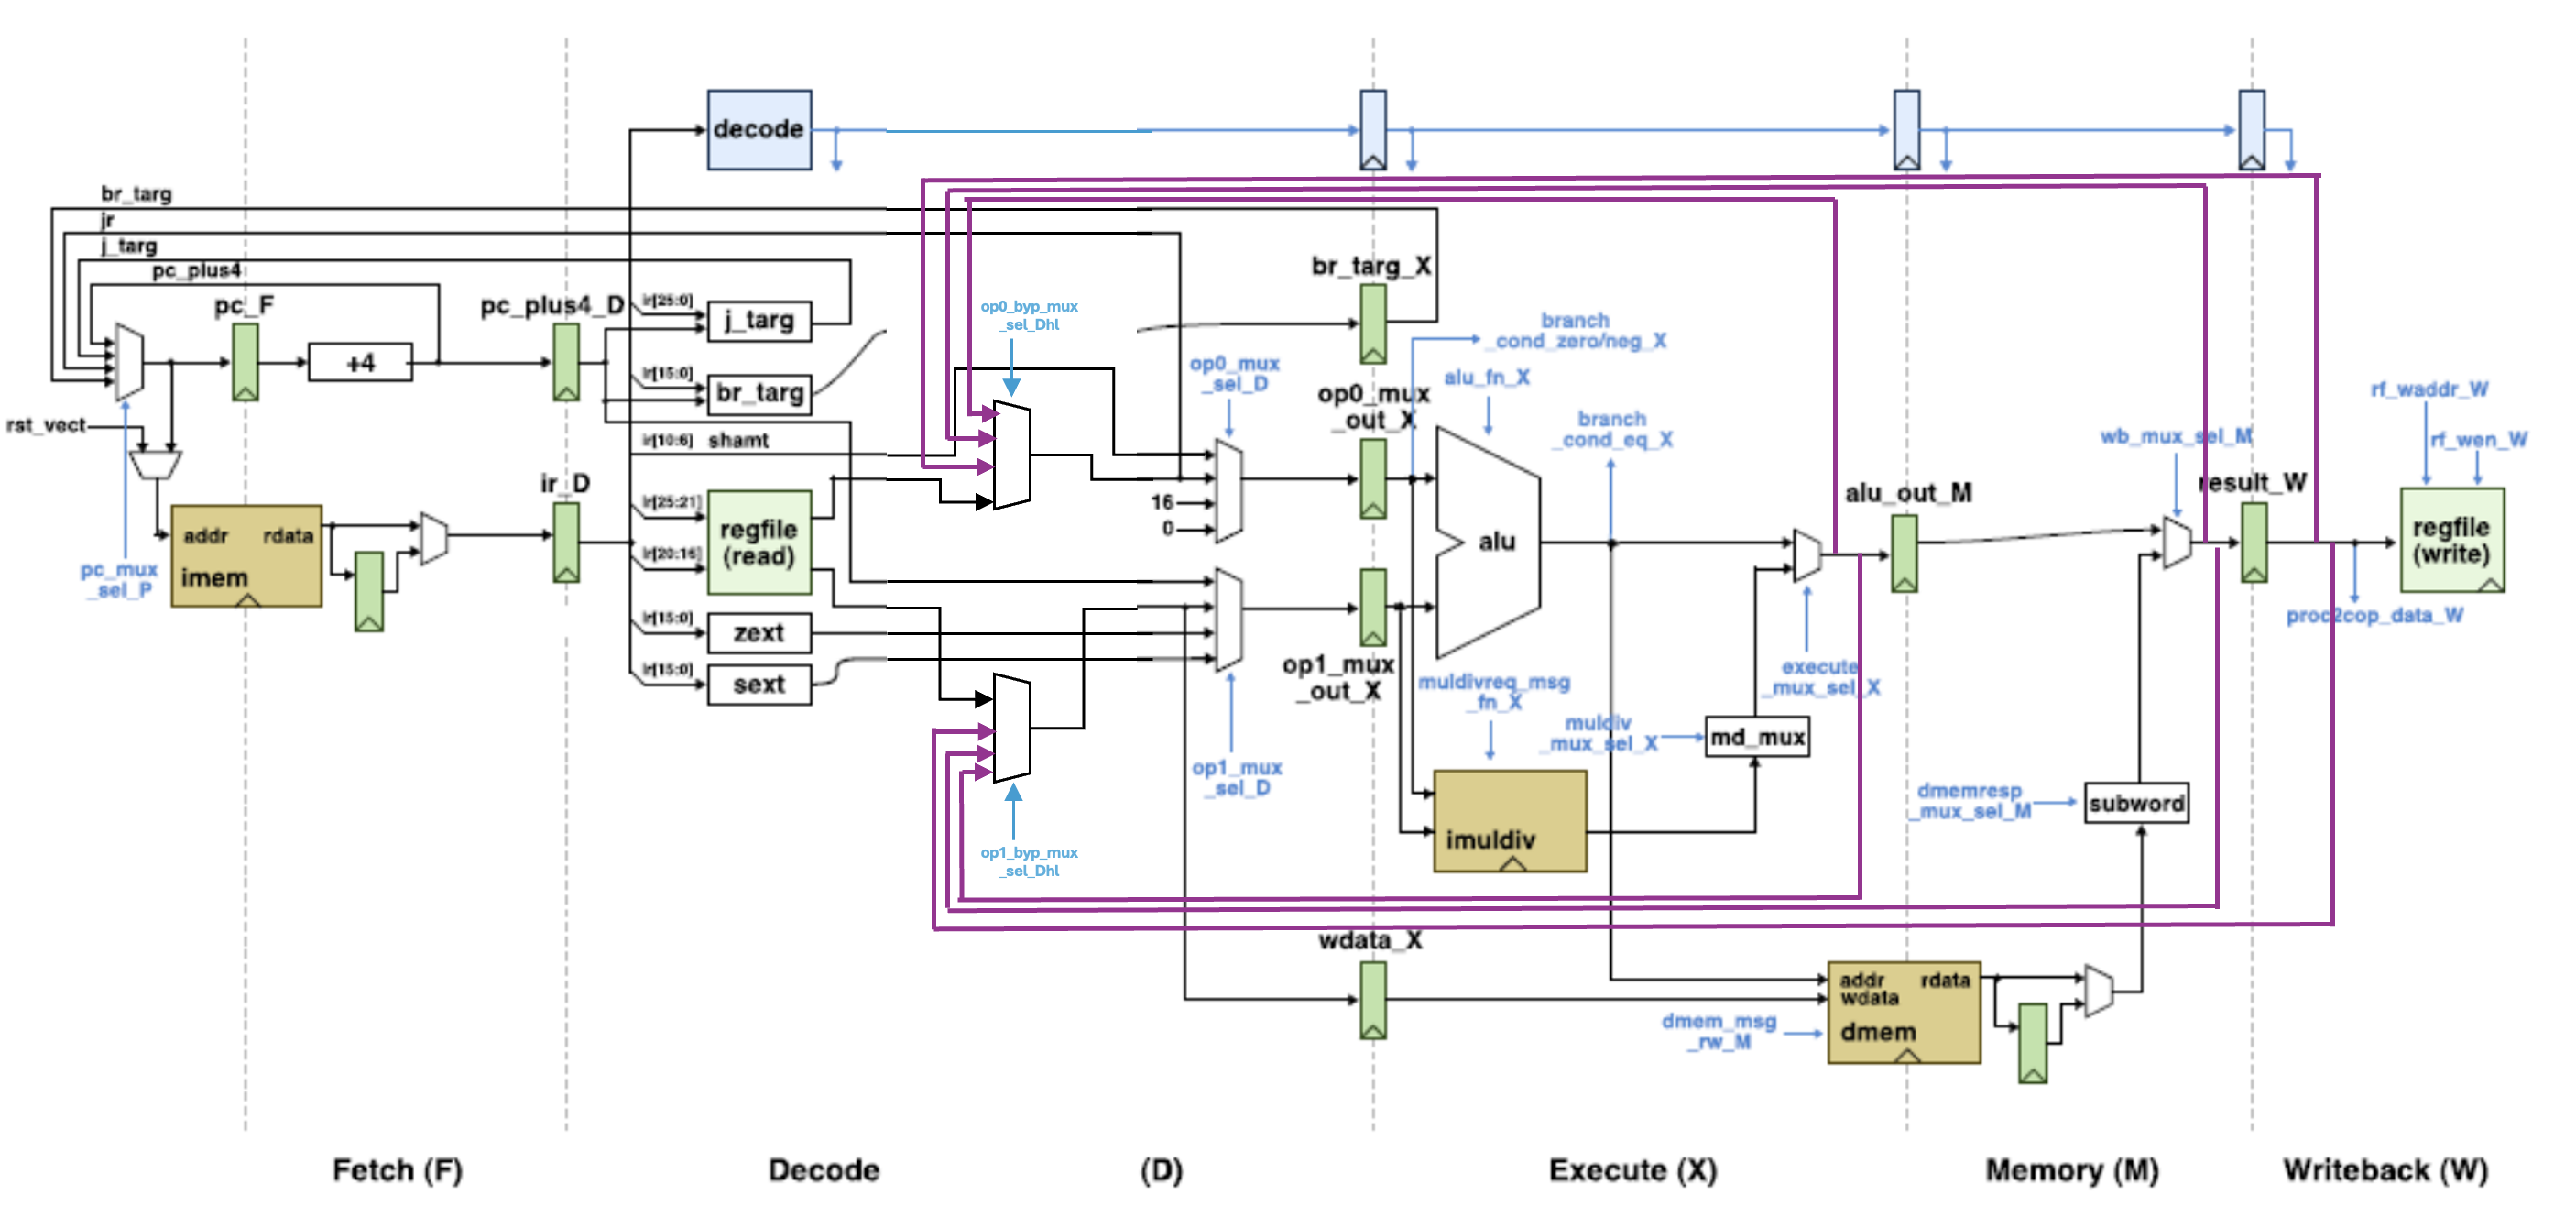
\includegraphics[scale=0.32]{../lab2_bypdpath.png}
Figure 1: PARCv2 datapath with bypassing.
\end{center}

\vspace{0.3cm}
%See the new muxes within the Decode stage, one for op0 and one for op1. 

\begin{center}
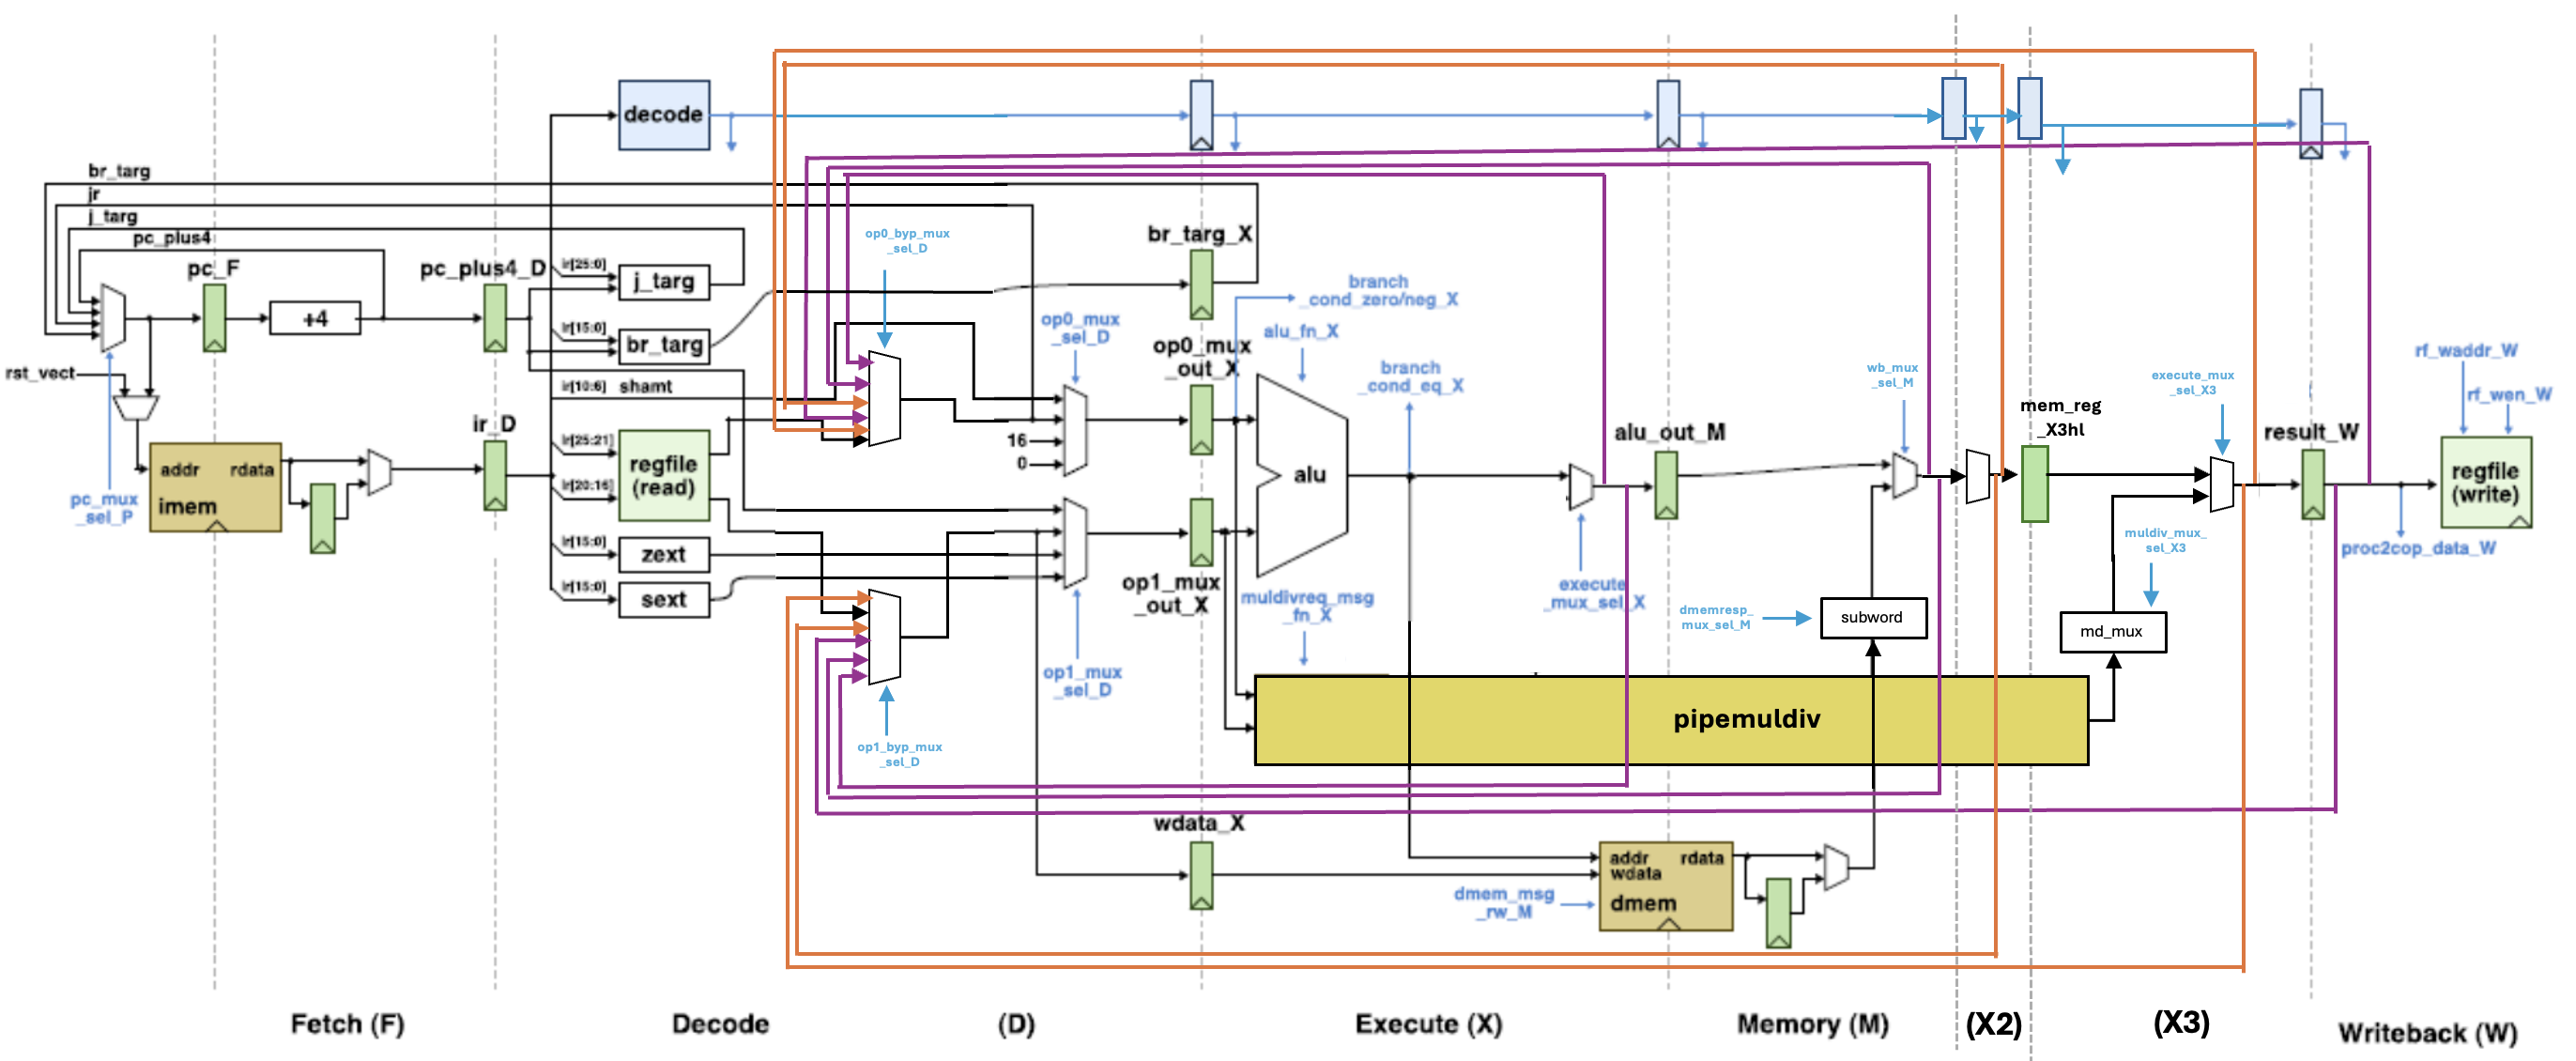
\includegraphics[scale=0.28]{../lab2_longdpath.png}
Figure 2: PARCv2 datapath with pipelined muldiv unit, with appropriate stalling and bypassing. 
\end{center}



\end{document}


